\subsection{Datasets}

All the input files we used consist of edges making it straightforward to parse them as showed in Figure \ref{fig:graphfileformat}.

\begin{verbbox}
node_from_1 node_to_1
node_from_2 node_to_2
...
node_from_n node_to_n
\end{verbbox}

\begin{figure}[ht]
  \centering
  \theverbbox
  \caption{Graph file format}
  \label{fig:graphfileformat}
\end{figure}

We used different graph files taken from \cite{datasets} to measure both the Sequential and Map-Redude algorithm performance. The following table describes different metrics of each one:

\begin{table}[h!]
\footnotesize
\begin{center}
\begin{tabular}{|c|c|c|c|}
\hline
{\bf Name} & {\bf Nodes}& {\bf Edges} & {\bf Size}\\
\hline
\hline
simple\_graph   & 10  & 14  & 55 bytes  \\
\hline
medium\_graph   & 534  & 9626  & 96.2 Kb  \\
\hline
ego-Facebook   & 4039  & 88234  & 854.4 Kb  \\
\hline
ego-Gplus   & 107614  & 13673453  & 1.2GB  \\
\hline
big\_graph   & 19670319  & 146213222  & 2.4GB  \\
\hline
\end{tabular}
\caption{Graphs}
\label{tb:graphfiles}
\end{center}
\end{table}

\subsection{Sequential}
We used an implementation of Tarjan's Algorithm that has $O(|V| + |E|)$ worst case performance. It uses a Depth-First-Approach (DFS) as described in Section \ref{sec:algo}. It begins at an arbitrary node and  visits every node of the graph exactly once. As it is going through the graph it will be generating the various connected components.

\begin{table}[!h]
\scriptsize
\begin{center}
\begin{tabular}{|c|c|c|c|}
\hline
{\bf Graph} & {\bf Parse (ms)} & {\bf Compute (ms)} & {\bf components \#} \\
\hline
\hline
simple\_graph   & 4  & 0.247 & 3 \\
\hline
medium\_graph   & 98  & 3 & 2 \\
\hline
ego-Facebook   & 232 & 14 & 1325  \\
\hline
ego-Gplus   & 49497 & 1104 & 37249 \\
\hline
big\_graph   & ?  & ? & ?  \\
\hline
\end{tabular}
\caption{Sequential times}
\label{tb:sequentialtimes}
\end{center}
\end{table}

The results here are as expected. The algorithm performs really well when using small files and the total execution time is really small. However, we can see that as the files grow bigger and bigger the parsing time starts becoming the dominating factor that takes up most of the total execution time. The big graph instance was not successfully run on a single machine because of an out-of-memory error. The next step is to try with a really big virtual machine in AWS with enough memory that can handle it.

\subsection{Map-Reduce}

Table \ref{tb:MapReducetimes} contains the execution time for the Map-Reduce implementation for each input graph file. We can see that using Map-Reduce for really small files is not very efficient but the real advantage is when using it to process large files. Specifically,  using Map-Reduce we were able to process the big\_graph file which failed on a single machine due to memory limitations.

\begin{table}[h!]
\footnotesize
\begin{center}
\begin{tabular}{|c|c|c|}
\hline
{\bf Graph} & {\bf Phase 1 (sec)} & {\bf Phase 2 (sec)}\\
\hline
\hline
simple\_graph   & 23  & 82 \\
\hline
medium\_graph   & 25 & 115 \\
\hline
ego-Facebook   & 25 & 180 \\
\hline
ego-Gplus   & 67  & 193 \\
\hline
big\_graph   & 153 & 1840 \\
\hline
\end{tabular}
\caption{Map-Reduce times}
\label{tb:MapReducetimes}
\end{center}
\end{table}

Figure \ref{fig:mapreduce_graph} shows an overview of the times it took us to run the Map-Reduce jobs for the different graphs. It is obvious that the parsing time now is linear to the size of input since it is being split among the multiple mappers. This is one advantage of Map-Reduce. We can also observe that using Map-Reduce for small graphs is more of an actual overhead rather than helpful. However, when it comes to large graphs Map-Reduce performs really well and it is possible to even parse the big graph successfully. The pattern here suggests that even when the graph becomes bigger the first phase is linear to the size of the input, while the second phase depends on the input and specifically, on how many rounds of Map-Reduce are performed.

\begin{figure}[!h]
 \centering
    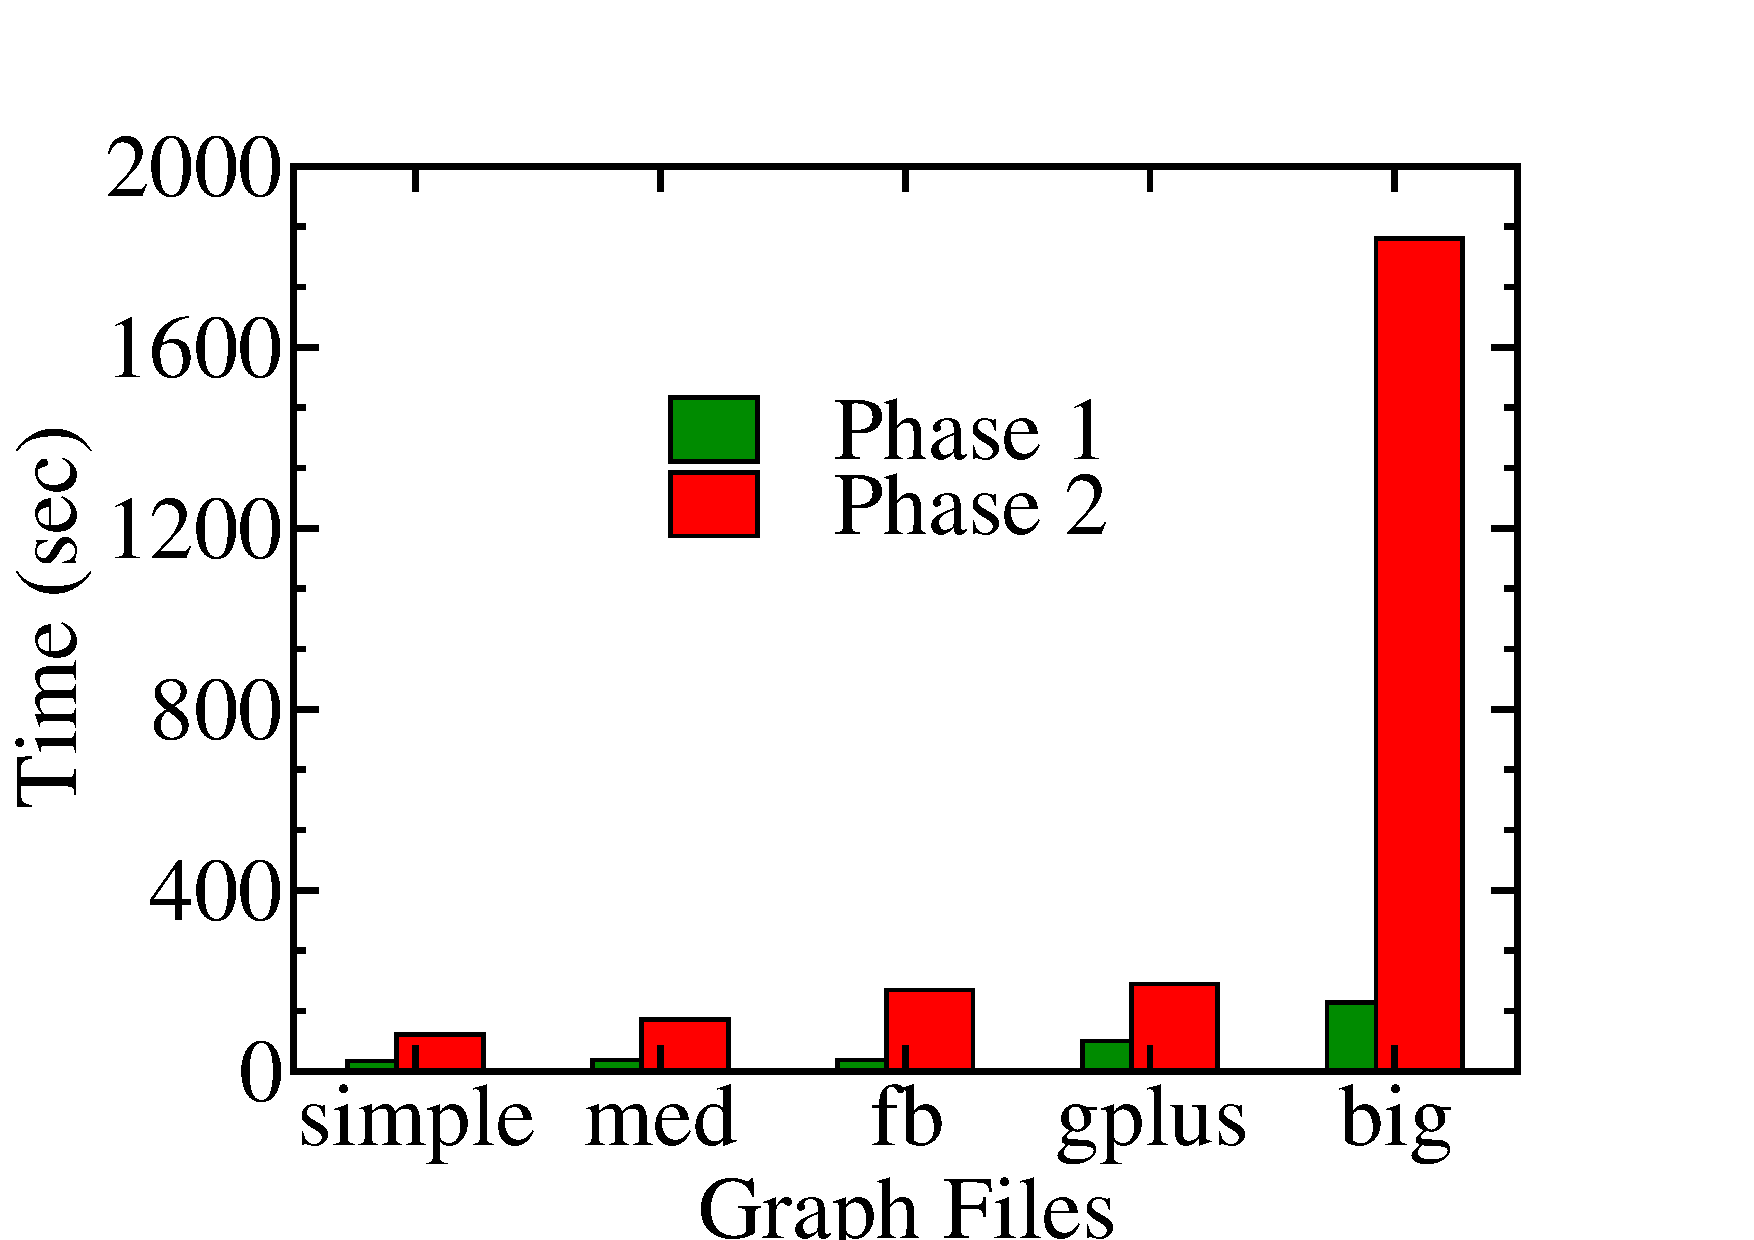
\includegraphics[]{figures/mapreduce_graph}
	\caption{Map-Reduce running times}
    \label{figure:mapreduce_graph}
\end{figure}

